\documentclass{article}

% if you need to pass options to natbib, use, e.g.:
% \PassOptionsToPackage{numbers, compress}{natbib}
% before loading nips_2017
%
% to avoid loading the natbib package, add option nonatbib:
% \usepackage[nonatbib]{nips_2017}

\usepackage[nonatbib]{nips_2017}

% to compile a camera-ready version, add the [final] option, e.g.:
% \usepackage[final]{nips_2017}

\usepackage[utf8]{inputenc} % allow utf-8 input
\usepackage[T1]{fontenc}    % use 8-bit T1 fonts
\usepackage{hyperref}       % hyperlinks
\usepackage{url}            % simple URL typesetting
\usepackage{booktabs}       % professional-quality tables
\usepackage{amsfonts}       % blackboard math symbols
\usepackage{nicefrac}       % compact symbols for 1/2, etc.
\usepackage{microtype}      % microtypography

\usepackage{mathtools}
\usepackage{graphicx}
\usepackage[ruled,linesnumbered]{algorithm2e}
\usepackage{multirow}
\usepackage{subcaption}
\usepackage{alphalph}
\usepackage{xr}
\usepackage{amsmath}
\usepackage{floatrow}

\floatsetup[subfigure]{capbesideposition={left,center}}
\externaldocument[J-]{supplementary_note}
\renewcommand{\thesubfigure}{\thesection.\arabic{subfigure}}
\DeclareMathOperator*{\argmax}{arg\,max}
\DeclareMathOperator*{\undermax}{max}
\DeclareMathOperator*{\undermin}{min}

\title{Temporal Coherence based Criteria for Predicting the Future using Deep Multi-stage Generative Adversarial Networks}

% The \author macro works with any number of authors. There are two
% commands used to separate the names and addresses of multiple
% authors: \And and \AND.
%
% Using \And between authors leaves it to LaTeX to determine where to
% break the lines. Using \AND forces a line break at that point. So,
% if LaTeX puts 3 of 4 authors names on the first line, and the last
% on the second line, try using \AND instead of \And before the third
% author name.

\author{
  Prateep Bhattacharjee \\
  Department of Computer Science\\
  Indian Institute of Technology Madras\\
  Chennai-600036, India \\
  \texttt{prateepb@cse.iitm.ac.in}
  %% examples of more authors
   \And
   Sukhendu Das \thanks{Webpage: http://www.cse.iitm.ac.in/~sdas/} \\
   Department of Computer Science\\
   Indian Institute of Technology Madras \\
   Chennai-600036, India \\
   \texttt{sdas@iitm.ac.in} \\
}

\begin{document}
% \nipsfinalcopy is no longer used

\maketitle

\begin{abstract}
  Predicting the future from a sequence of video frames has been recently a sought after yet challenging task in the field of computer vision and machine learning. Although there have been efforts for tracking using motion trajectories and flow features, the problem of generating unseen frames has not been studied extensively. In this paper, we deal with this problem using convolutional models inside a multi-stage Generative Adversarial Networks (GAN) framework.
  The proposed method uses two stages of GANs to generate crisp and clear set of future frames. Although GANs have been used in the past for predicting the future, none of the works consider relation between subsequent frames in the temporal dimension. Our main contribution lies in formulating two objective functions based on the Normalized Cross Correlation (NCC) and the Pairwise Contrastive Divergence (PCD). This method, coupled with the traditional L1 loss, is tested on three real world video datasets \textit{viz.} Sports-1M, UCF-101 and the KITTI. Performance analysis reveals superior results over the recent state-of-the-art methods.
\end{abstract}

\section{Introduction}
  Video frame prediction has always been one of the fundamental problems in computer vision as it caters to a wide range of applications including self-driving cars, surveilance, robotics and inpainting. However, the challenge lies in the fact that, real-world scenes tend to be complex, and predicting the future events requires modelling of complicated internal representations of the ongoing events. Recently, the work of \cite{mathieu2015deep} modeled this problem in the framework of Generative Adversarial Networks (GAN). Generative models, as introduced by Goodfellow \textit{et. al.}, \cite{goodfellow2014generative} try to generate images from random noise by simultaneously training a generator (G) and a discriminator network (D) in a process similar to a zero-sum game. Mathieu \textit{et. al.} \cite{mathieu2015deep} shows the effectiveness of this adversarial training in the domain of frame prediction using a combination of two objective functions (along with the basic adversarial loss) employed on a multi-scale generator network. This idea stems from the fact that the original $ L2 $-loss tends to produce blurry frames. This was overcome by the use of Gradient Difference Loss (GDL) \cite{mathieu2015deep}, which showed significant improvement over the past approaches when compared using similarity and sharpness measures. However, this approach, although producing satisfying results for the first few predicted frames, tends to generate blurry results for predictions far away ($ \sim $6) in the future. 
  
  In this paper, we aim to get over this tendency of producing blurry predictions by taking into account the relation between consecutive frames in the temporal dimension also. We propose two objective functions: (a) \textbf{Normalized Cross-Correlation Loss (NCCL)} and (b) \textbf{Pairwise Contrastive Divergence Loss (PCDL)} for effectively capturing inter-frame relationships in the GAN framework.
  NCCL maximizes the cross-correlation between neighbourhood patches from consecutive frames whereas, CDL applies a penalty when subsequent generated frames are predicted wrongly by the discriminator network (D), thereby separating them far apart in the feature space. 
  
  The rest of the paper is organized as follows: section \ref{sec:model} describes the multi-stage generative adversarial arhitecture used, the sections \ref{sec:nccl} - \ref{sec:combloss} introduce the different loss funtions employed: the adversarial loss (AL), $ L2 $-loss (L2) and most importantly NCCL and CDL. We show the results of our experiments on Sports-1M \cite{KarpathyCVPR14}, UCF-101 \cite{soomro2012ucf101} and KITTI \cite{Geiger2013IJRR} and compare them with state-of-the-art techniques in section \ref{sec:experiments}. Finally, we conclude our paper highlighting the key points and future direction of research in section \ref{sec:conclusion}.

\section{Multi-stage Generative Adversarial Model}
  \label{sec:model}
  
  \begin{figure}[t]
  	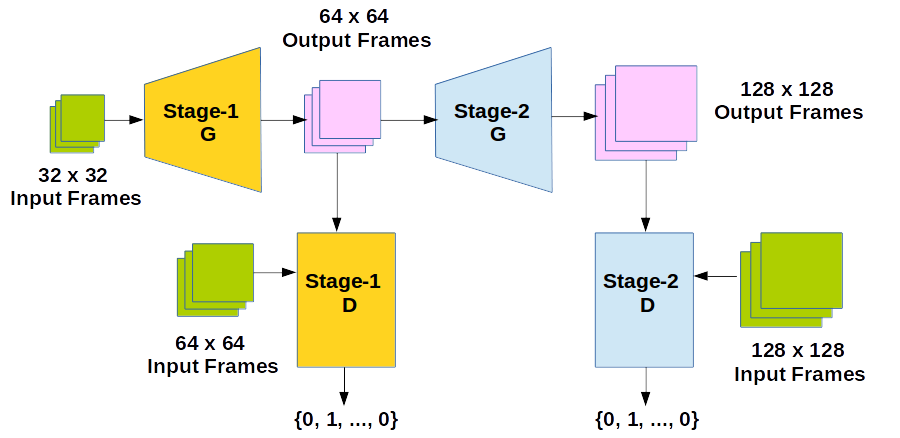
\includegraphics[scale = 0.45]{Images/multi_gan.png}
  	\caption{The proposed multi-stage GAN framework. The stage-1 generator network outputs a low-resolution version of predicted frames which are then fed through the stage-2 generator. Discriminators at both the stages predict $ 0 $ or $ 1 $ per predicted frame to denote its origin: synthetic or original.}
  	\label{fig:gan}
  \end{figure}
  Generative Adversarial Networks (GAN) \cite{goodfellow2014generative} are composed of two networks: (a) the Generator (G) and (b) the Discriminator (D). The generator G tries to generate realistic images by learning to model the true data distribution $ p_{data} $ and thereby trying to make the task of differentiating between original and generated images by the discriminator difficult. The discriminator D, in the other hand, is optimized to distinguish between the synthetic and the real images. In essence, this procedure of alternate learning is similar to the process of two player min-max games \cite{goodfellow2014generative}. Overall, the GANs try to minimize the following objective function
  \begin{equation}
  	\undermin_G \undermax_D v(D, G) = \mathbb{E}_{x \sim p_{data}} [log (D(x))] + \mathbb{E}_{z \sim p_z} [log (1 - D(G(z)))]
  	\label{eq:gan}
  \end{equation}
  where, $ x $ is a real image from the true distribution $ p_{data} $ and $ z $ is a vector sampled from the distibution $ p_z $, usually uniform or Gaussian. The adversarial loss employed in this paper is slightly different from equation \ref{eq:gan}, as, the input to our network is a sequence of frames of a video, instead of a noise vector $ z $. 
  
  As convolutions account only for short-range relationships, pooling layers are used to garner information from wider range. But, this process generates low resolution images. To overcome this, Mathieu \textit{et. al.} \cite{mathieu2015deep} uses a multi-scale generator network, equivalent to the reconstruction process of a Laplacian pyramid \cite{DBLP:journals/corr/RadfordMC15}, coupled with discriminator networks to produce high-quality output frames of size $ 32 \times 32 $.
  There are two shortcomings of this approach:
  \renewcommand{\theenumi}{\alph{enumi}} 
  \begin{enumerate}
  	\item Generating image output at higher dimensions \textit{viz.} $ (128 \times 128) $ or $(256 \times 256) $, requires multiple use of some statc upsampling operator applied on the output of the generators. In our proposed model, this upsampling is handled by the generator models implicitly through the use of consecutive unpooling operations, thereby generating predicted frames at much higher resolution in lesser number of scales.
  	
  	\item  As the generator network parameters are not learned with respect to any objective function which captures the temporal relationship effectively, the output becomes blurry after $ \sim 4 $ frames.
  \end{enumerate}
  
  To overcome the first issue, we propose a multi-stage ($ 2 $-stage) generative adversarial network.
  
  \subsection{Stage-1}
	  Generating the output frame(s) directly often produces blurry outcomes. Instead, we simplify the process by first generating crude, low-resolution version of the frame(s) to be predicted. The stage-1 generator ($ G_1 $) consists of a series of convolutional layers coupled with unpooling layers \cite{zeiler2014visualizing} which upsample the frames. We used ReLU non-linearity in all but the last layer, in which case, tanh was used following the scheme of \cite{DBLP:journals/corr/RadfordMC15}. The inputs to $ G_1 $ are $ m $ number of consecutive frames of dimension $ W_0 \times H_0 $, whereas the outputs are $ n $ predicted frames of size $ W_1 \times H_1$, where, $ W_1 = W_0 \times 2 $ and $ H_1 = H_0 \times 2 $. These outputs, stacked with the upsampled version of the original input frames, produce the input of dimension $ (m + n) \times W_1 \times H_1 $ to the stage-1 discriminator ($ D_1 $). $ D_1 $ applies a chain of convolutional layers followed by multiple fully-connected layers to finally produce an output vector of dimension $ (m + n) $, consisting of $ 0 $'s and $ 1 $'s. 
	  
	  One of the key differences of our proposed GAN framework is that, the discriminator network produces decision output for multiple frames, instead of a single $ 0/1 $ outcome. This is exploited by one of the proposed objective functions, the CDL, which is described in later sections.
  
  \subsection{Stage-2}
	  The second stage network closely resembles the stage-1 architecture, with difference only in the input and output dimensions. The input to the stage-2 generator ($ G_2 $) is formed by stacking the predicted frames and the upsampled inputs of $ G_1 $, thereby having dimension of $ (m + n) \times W_1 \times H_1 $.
	  The output of $ G_2 $ are $ n $ predicted high-resolution frames of size $ W_2 \times H_2 $, where, $ W_2 = W_0 \times 4 $ and $ H_2 = H_0 \times 4 $. The stage-2 discriminator ($ D_2 $), works in similar fashion as $ D_1 $, producing output vector of length $ (m + n) $.
	  
	  Effectively, the multi-stage model can be represented by the following recursive equations:
	  \begin{equation}
	  	Y_k = \left\{\begin{alignedat}{2}
	  	& G_k(Y_{k-1}, X_{k-1}), \quad & for \quad k \geq 2 \\ & G_k(X_{k-1}) &  for \quad k = 1
	  	\end{alignedat}\right.
	  	\label{eq:multi-gan}
	  \end{equation}
	  where, $ Y_k $ is the set of predicted frames, $ X_k $ are the input frames at the $ k $th stage of the generator network $ G_k $.
  
\subsection{Training the multi-stage GAN}
  The training procedure of the multi-stage GAN model follows that of the original generative adversarial networks with minor variations. The training of the discriminator and the generator are described as follows:
  \paragraph{Training of the discriminator} Considering the input to the discriminator ($ D $) as $ X $ (series of $ m $ frames) and the target output to be $ Y $ (series of $ n $ frames), $ D $ is trained to distinguish between synthetic and original inputs by classifying $ (X, Y) $ into class 1 and $ (X, G(X)) $ into class 0. Hence, for each of the stages $ k $, we train $ D $ with target $ \vec{1} $ (Vector of $ 1 $'s with dimension $ m $) for $ (X, Y) $ and target $ \vec{0} $ (Vector of $ 0 $'s with dimension $ n $) for $ (X, G(X)) $. The loss function for training $ D $ can be described as follows:
  \begin{equation}
  	\mathcal{L}_{adv}^D = \sum_{k = 1}^{N_{stages}} L_{bce}(D_k(X_k, Y_k), \vec{1}) + L_{bce}(D_k(X_k, G_k(X_k)), \vec{0})
  	\label{eq:gan_d}
  \end{equation}
  where, $ L_{bce} $, the binary cross-entropy loss can be defined as:
  \begin{equation}
  	L_{bce}(Y, Y') = - \sum_{i = 1}^{|Y|} Y^{'i} log(Y^i) + (1 - Y^{'i}) log (1 - Y^i), Y^i \in \{0,1\}, Y^{'i} \in [0,1]
  	\label{eq:gan_bce} 
  \end{equation}
	
  \paragraph{Training of the generator} We perform an optimization step on the generator network ($ G $), keeping the weights of $ D $ fixed, by feeding a set of consecutive frames $ X $ sampled from the training data with target $ Y $ (set of ground-truth output frames) and minimize the following adversarial loss:
  \begin{equation}
  	\mathcal{L}_{adv}^G = \sum_{k = 1}^{N_{stages}} L_{bce}(D_k(X_k, G_k(X_k)), \vec{1})
  	\label{eq:gan_g}
  \end{equation}
  
  By minimizing the above two losses (eqn. \ref{eq:gan_d}, \ref{eq:gan_g}), $ G $ tries to make the discriminator believe that, the source of the generated frames is the input data space itself. Although this alternate optimization of $ D $ and $ G $ is theoretically correct, in practical purposes, this produces an unstable system where $ G $ can produce samples that consecutively move far away from the original input space and in consequence $ D $ distinguishes them easily. To overcome this unstability inherent in the GAN principle, and to make much clear and crisp predicted frames at high resolution, we add two more objective functions: (a) Normalized Cross Correlation Loss (NCCL) and (b)Pairwise Contrastive Divergence Loss (PCDL) to the original adversarial loss (refer to eqn. \ref{eq:gan_d} and \ref{eq:gan_g}).  

\section{Normalized Cross-Correlation Loss (NCCL)}
  \label{sec:nccl}
  The main advantage of video over image data is the fact that, it offers a far richer space of data distribution by adding the temporal dimension along with the spatial one. Convolutional Neural Networks (CNN) can only capture short-range relationships, a small part of the vast available information, from the input video data, that too in the spatial domain. Although this can be somewhat alleviated by the use of 3D convolutions \cite{ji20133d}, this increases the number of learnable parameters by a large scale. Normalized cross-correlation has been used since long time in the field of video analytics \cite{bovik2009essential, briechle2001template, nakhmani2013new, luo2010fast} to model the space-time relationships present in the data.
  
  Normalized cross correlation (NCC) measures the similarity of two image patches as a function of the displacement of one relative to the other. This can be mathematically defined as
  \begin{equation}
  	NCC(f, g) = \sum_{x, y}^{}\frac{(f(x, y) - \mu_f)(g(x, y) - \mu_g)}{\sigma_f \sigma_g}
  	\label{eq:ncc}
  \end{equation}
  where, $ f(x, y) $ is a subimage, $ g(x, y) $ is the template to be matched, $ \mu_f, \mu_g $ denotes the mean of the subimage and the template respectively and $ \sigma_f, \sigma_g $ denotes the standard deviation of $ f $ and $ g $ respectively.
  
  In the domain of video frame(s) prediction, we incorporate the NCC by first extracting small non-overlapping square patches of size $ h \times h $ ($ 1 < h \leq 4 $), denoted by a 3-tuple $ P_t\{x, y, h\} $, where, $ x $ and $ y $ are the co-ordinates of the top-left pixel of a particular patch, from the predicted frame at time $ t $ and then calculating the cross-correlation score with the patch extracted from the ground truth frame at time $ (t-1) $, represented by $ \hat{P}_{t-1}\{x-2, y-2, h+4\} $. 
  
  In simpler terms, we aim to find the cross-correlation score between a small portion of the current predicted frame and the local neighborhood of that in the previous ground-truth frame. We assume that, the motion present in the full frame can be subdivided into smaller parts and can be effectively approximated by looking into small local neighborhoods in the temporal dimension. This stems from the fact that, unless the video contains significant jitter or unexpected random events like scene change, the motion features remain smooth over time. The step-by-step process for finding the cross-correlation score by matching local patches of predicted and ground truth frames is described in algorithm \ref{algo:ncc}.
  
  The idea of calculating the NCC score can be effectively modeled into an objective function for the generator network $ G $, where, it tries to maximize the score over a batch of inputs. In essence, this objective funtion tries to model the temporal data distribution by smoothing the local motion features generated by the convolutional model. This loss function, $ \mathcal{L}_{NCC} $ can be defined as
  \begin{equation}
  	\mathcal{L}_{NCC} = \sum_{batch = 1}^{N}Score_{NCC}
  	\label{eq:lncc}
  \end{equation}
  where, $ batch $ denotes a minibatch of input frames and $ Score_{NCC} $, obtained using algorithm \ref{algo:ncc}, is the average normalized cross-correlation score per batch. The generator tries to maximize $ \mathcal{L}_{NCC} $ along with the adversarial loss defined in section \ref{sec:model}. 
  
  We also propose a variant of this objective function, termed as Smoothed Noralized Cross-Correlation Loss (SNCCL), where the patch similarity finding logic of NCCL is extended by convolving with Gaussian filters to suppress small sudden motion pattern changes. This algorithm is discussed in sec. A of the supplementary document for space restrictions.  
  
  \begin{algorithm}[!htbp]
  	\SetAlgoLined
  	\KwIn{Ground-truth frames $ (GT) $, Predicted frames $ (PRED) $}
  	\KwOut{Cross-correlation score ($Score_{NCC}$)}
  	\textbf{Variables:}\\
  	$ h $ = height and width of an image patch\\
  	$ t $ = current time\;
  	\textbf{Initialize:} $ Score_{NCC} = 0 $\;
  	\For{$ t = 1 $ upto $ T $}{
  		\For{$ i = 0 $ upto $ H $, $ i \leftarrow i + h $}{
	  		\For{$ j = 0 $ upto $ H $, $ j \leftarrow j + h $}{
	  			$ P_t \leftarrow extract\_patch(PRED_t, i, j, h) $\;
	  			$ \backslash \backslash $ Extracts a patch from the predicted frame at time $ t $ of dimension $ h \times h $ starting from the top-left pixel index $ (i,j) $\;
	  			$ \hat{P}_{t - 1} \leftarrow extract\_patch(GT_{t - 1}, i - 2, j - 2, h + 4) $\;
	  			$ \backslash \backslash $ Extracts a patch from the ground-truth frame at time $ (t-1) $ of dimension $ (h+4) \times (h+4) $ starting from the top-left pixel index $ (i-2,j-2) $\;
	  			$ \mu_{P_t} \leftarrow avg(P_t)$\;
	  			$ \mu_{\hat{P}_{t-1}} \leftarrow avg(\hat{P}_{t-1})$\;
	  			$ \sigma_{P_t} \leftarrow standard\_deviation(P_t)$\;
	  			$ \sigma_{\hat{P}_{t-1}} \leftarrow standard\_deviation(\hat{P}_{t-1})$\;
	  			$ Score_{NCC} \leftarrow Score_{NCC} + Absolute\big(\sum_{x, y}^{}\frac{(P_t(x, y) - \mu_{P_t})(\hat{P}_{t-1}(x, y) - \mu_{\hat{P}_{t-1}})}{\sigma_{P_t} \sigma_{\hat{P_{t-1}}}} \big)$\;
	  		}	
  		}
  	}
  	$ Score_{NCC} \leftarrow avg(Score_{NCC}) $\;
  \caption{Calculation of the normalized cross-correlation score for finding similarity between a set of predicted frame(s) and a set of ground-truth frame(s).}
  \label{algo:ncc}
\end{algorithm}

\section{Pairwise Contrastive Divergence Loss (PCDL)}
  \label{sec:pcdl}
  As discussed in sec. \ref{sec:nccl}, the proposed method tries to capture motion features that vary slowly over time. The NCCL aims to achieve this using local similarity measures. To complement this in a global scale, we use the idea of pairwise contrastive divergence over the input frames. The idea of exploiting this temporal coherence for learning motion features has been studied in the recent past \cite{goroshin2015unsupervised, hadsell2006dimensionality,  mobahi2009deep}.
  
  By assumming that, motion features vary slowly over time, we describe $ \hat{Y}_t $ and $ \hat{Y}_{t-1} $ as a temporal pair, where, $ \hat{Y}_i $ and $ \hat{Y}_{t-1} $ are the predicted frames at time $ t $ and $ (t-1) $ respectively, if the outputs of the discriminator network $ D $ for both these frames are $ 1 $. With this notation, we model the slowness principle of the motion features using an objective function as
  \begin{equation}
	  \begin{split}
		  \mathcal{L}_{PCDL} & = \sum_{i = 0}^{T} D_{\delta}(\hat{Y}_i, \hat{Y}_{i + 1}, p_i) \\
		  & = \sum_{i = 0}^{T} p_i d(\hat{Y}_i, \hat{Y}_{i + 1}) + (1 - p_i) max(0, \delta - d(\hat{Y}_i, \hat{Y}_{i + 1}))
	  \end{split}
	  \label{eq:pcdl}
  \end{equation}   
  where, $ T $ is the time-duration of the frames predicted, $ p_i $ is the output decision ($p_i \in \{0, 1\} $) of the discriminator, $ d(x, y) $ is a distance measure ($ L2 $ in this paper) and $ \delta $ is the margin. Equation \ref{eq:pcdl}, in simpler terms, tries to minimize the distance between frames that have been predicted correctly and encourages the distance in the negative case, upto a margin $ \delta $.
  
  PCDL can be extended upto higher order versions, taking into account triplets or $ n $ number of predicted frames instead of the general pairwise case. We discuss about higher order versions (especially when $ n = 3 $) in sec. B of the supplementary document.
\section{Combined Loss}
\label{sec:combloss}
Finally, we combine the objective functions described in eqn. \ref{eq:gan_g} - \ref{eq:pcdl} along with the general $ L1 $-loss with different weights as
\begin{equation}
	\begin{split}
	\mathcal{L}_{Combined} = & 	\lambda_{adv}\mathcal{L}_{adv}^G (X, Y) + \lambda_{L1} \mathcal{L}_{L1} (X, Y) \\
	& + \lambda_{NCCL} \mathcal{L}_{NCCL} (X, Y) + \lambda_{PCDL} \mathcal{L}_{PCDL} (X, Y)
	\end{split}
	\label{eq:combined}
\end{equation}
For the sake of simplicity, all the weights \textit{viz.} $\lambda_{L1}, \lambda_{NCCL} $ and $ \lambda_{PCDL} $ have been set as 1, while $ \lambda_{adv} $ equals $ 0.05 $ for all the experimental studies. This overall loss is minimized during the training stage of the multi-stage GAN using Adam optimizer \cite{kingma2014adam}. 

\section{Experiments}
  \label{sec:experiments}
  Experimental studies of our video frame(s) prediction model have been carried out on video clips from Sports-1m, UCF-101 \cite{soomro2012ucf101} and KITTI \cite{Geiger2013IJRR}. The input-output configuration used for training the system is as follows: \textbf{input}: 4 frames and \textbf{output}: 6 frames. We compare our results to recent state-of-the-art methods by computing two popular metrics: (a) \textbf{Peak Signal to Noise Ratio (PSNR)} and (b) \textbf{Structural Similarity Index Measure (SSIM)} \cite{wang2004image}.

\subsection{Datasets}
  \paragraph{Sports-1M} A large collection of sports videos collected from YouTube spread over 487 classes. The main reason for chosing this dataset is the amount of movement in the frames. Being a collection of sports videos, this has sufficient amount of motion present in most of the frames, making it an efficient dataset for training the prediction model.
  \paragraph{UCF-101} This dataset contains $ 13320 $ annotated videos belonging to 101 classes having 180 frames/video on average. The frames in this video do not contain as much movement as the Sports-1m and hence this is used only for testing purpose.
  \paragraph{KITTI} This consists of high-resolution video data from different road conditions. We have taken raw data from two categories: (a) city and (b) road.

\subsection{Architecture of the network}

  \begin{table}[!htbp]
  	\caption{Network architecture details. $ G $ and $ D $ represents the generator and discriminator networks respectively. $ U $ denotes an unpooling operation which upsamples an input of dimension $ h \times h $ into $ (h \times 2) \times (h \times 2) $.}
  	\centering
  	\begin{tabular}{p{2.3cm}p{3cm}p{2.5cm}p{2cm}p{2cm}}
  		\hline
  		Network & Stage-1 (G) & Stage-2 (G) & Stage-1 (D) & Stage-2 (D)\\
  		\hline
  		Number of feature maps & 64, 128, 256U, 128, 64 & 64, 128, 256, 512U, 256, 128, 64 & 64, 128, 256 & 128, 256, 512, 256, 128 \\
  		\hline
  		Kernel sizes & 5, 3, 3, 3, 5 & 5, 5, 5, 5, 5, 5 & 3, 5, 5  & 7, 5, 5, 5, 5  \\
  		\hline
  		Fully connected & N/A & N/A & 1024, 512 & 1024, 512 \\
  		\hline
  	\end{tabular}
  	\label{tab:arch}
  \end{table}

The architecture details for the generator (G) and discriminator (D) networks for experimental studies is shown in table \ref{tab:arch}. All the convolutional layers except the terminal one in both stages of $ G $ are followed by ReLU non-linearity. The last layer is tied with tanh activation function. In both the stages of $ G $, we use unpooling layers to upsample the image into higher resolution in magnitude of $ 2 $ in both dimensions (height and width). The learning rate is set to $ 0.003 $ for $ G $, which is gradually decreased to $ 0.0004 $ over time. The discriminator (D) uses ReLU non-linearities and is trained with a learning rate of $ 0.03 $. We use minibatches of 8 clips for training the overall network.

\subsection{Evaluation metric}
  Assesment of the quality of the predicted frames is done by two methods:
  (a) Peak Signal to Noise Ratio (PSNR) and (b) Structural Similarity Index Measure (SSIM).
  \textbf{PSNR} measures the quality of the reconstruction process through the calculation of Mean-squared error beteen the original and the reconstructed signal in logarithmic decibel scale \cite{bovik2009essential}.
  \textbf{SSIM} is also an image similarity measure where, one of the images being compared is assumed to be of perfect quality \cite{wang2004image}.
  
  As the frames in videos are composed of foreground and background, and in most cases the background is static (not the case in the KITTI dataset, as it has videos taken from camera mounted on a moving car), we extract random sequences of $ 32 \times 32 $ patches from the frames with significant motion. Calculation of motion presence is done by the use of optical flow method of \textit{Brox et. al.} \cite{brox2011large}.
  
\subsection{Comparison}
  We compare the results by testing on videos from UCF-101 using model trained on the Sports-1M dataset in table \ref{tab:ucf}. Superiority of our method over the most recent work \cite{mathieu2015deep} can be clearly detrmined from the comparison. We followed similar choice of test set videos as in \cite{mathieu2015deep} to make a fair comparison. One of the impressive facts in our model is that, it can produce acceptably good predictions even in the 4th frame, which is a significant result, considering the compared approach uses separate smaller models for achieving this feat. It is to be noted that, even though the metrics for the first predicted frame do not differ by a large margin compared to the results from \cite{mathieu2015deep}, the values decrease much slowly for the models trained with the proposed objective functions (rows 6-8 of table \ref{tab:ucf}). Our assumption for this phenomenon is the incorporation of the objective functions based on temporal relations also rather than only learning in the spatial domain. 
  
  \begin{table}[!htbp]
  	\centering
  	\caption{Comparison of different methods for the UCF-101 dataset. The first four rows report the results from \cite{mathieu2015deep}. (*) indicates models fine tuned on patches of size $ 64 \times 64 $ \cite{mathieu2015deep}. (-) denotes unavailability of data. GDL stands for Gradient Difference Loss \cite{mathieu2015deep}.}
  	\begin{tabular}{p{4cm}p{1cm}p{1cm}p{1cm}p{1cm}p{1cm}p{1cm}}
  		\hline
  		\multirow{2}{*}{} &
  		\multicolumn{2}{p{2.5cm}}{1st frame prediction scores} &
  		\multicolumn{2}{p{2.5cm}}{2nd frame prediction scores} &
  		\multicolumn{2}{p{2.5cm}}{4th frame prediction scores} \\
  		Methods & PSNR & SSIM & PSNR & SSIM & PSNR & SSIM \\
  		\hline
  		L1 & 28.7 & 0.88 & 23.8 & 0.83 & - & - \\
  		\hline
  		GDL L1 & 29.4 & 0.90 & 24.9 & 0.84 & - & - \\
  		\hline
  		GDL L1* & 29.9 & 0.90 & 26.4 & 0.87 & - & - \\
  		\hline
  		Adv + GDL fine-tuned* & 32.0 & 0.92 & 28.9 & 0.89 & - & - \\
  		\hline
  		Adv + NCCL + L1 & 35.4 & 0.94 & 32.9 & 0.92 & 22.7 & 0.64 \\
  		\hline
  		Adv + NCCL + PCDL & 37.1 & 0.95 & 34.5 & 0.92 & 23.4 & 0.69 \\
  		\hline
  		Adv + NCCL + PCDL + L1 & 37.3 & 0.95 & 34.7 & 0.92 & 23.6 & 0.69 \\
  		\hline
  		Adv + SNCCL + PCDL + 3-PCDL & 38.2 & 0.95 & 35.8 & 0.92 & 24.2 & 0.69 \\
  		\hline
  	\end{tabular}
  	\label{tab:ucf}
  \end{table}
   
   We also trained our model on the KITTI dataset and report the findings in table I of the supplementary document due to space restrictions.
   
   Finally, we show the prediction results obtained on both the UCF-101 and KITTI in fig. \ref{fig:big}. The results show only the first predicted frame for clear visibility. It is evident from the subfigures that, our proposed objective functions produce impressive quality frames while the models trained with L1 loss tends to output blurry reconstruction.
   
   
   
   \begin{figure}
   	\centering
   	\subcaptionbox{Input (t=0)\label{sfig:a}}{\includegraphics[width=.22\textwidth,height=2cm]{Images/Predictions/UCF/Demo_1/01.png}}\hfill
   	\subcaptionbox{Input (t=1)\label{sfig:b}}{\includegraphics[width=.22\textwidth,height=2cm]{Images/Predictions/UCF/Demo_1/02.png}}\hfill
   	\subcaptionbox{Input (t=2)\label{sfig:c}}{\includegraphics[width=.22\textwidth,height=2cm]{Images/Predictions/UCF/Demo_1/03.png}}\hfill
   	\subcaptionbox{Input (t=3)\label{sfig:d}}{\includegraphics[width=.22\textwidth,height=2cm]{Images/Predictions/UCF/Demo_1/04.png}}\
   	\subcaptionbox{Ground truth\label{sfig:e}}{\includegraphics[width=.22\textwidth,height=2cm]{Images/Predictions/UCF/Demo_1/gt.png}}\hfill
   	\subcaptionbox{Adv + L1\label{sfig:f}}{\includegraphics[width=.22\textwidth,height=2cm]{Images/Predictions/UCF/Demo_1/gen_adv.png}}\hfill
   	\subcaptionbox{Adv + NCCL\label{sfig:g}}{\includegraphics[width=.22\textwidth,height=2cm]{Images/Predictions/UCF/Demo_1/gen_pcdl.png}}\hfill
   	\subcaptionbox{Combined\label{sfig:h}}{\includegraphics[width=.22\textwidth,height=2cm]{Images/Predictions/UCF/Demo_1/gen_nccl.png}}\
   	
   	\subcaptionbox{Input (t=0)\label{sfig:i}}{\includegraphics[width=.22\textwidth,height=2cm]{Images/Predictions/UCF/Demo_2/01.png}}\hfill
   	\subcaptionbox{Input (t=1)\label{sfig:j}}{\includegraphics[width=.22\textwidth,height=2cm]{Images/Predictions/UCF/Demo_2/02.png}}\hfill
   	\subcaptionbox{Input (t=2)\label{sfig:k}}{\includegraphics[width=.22\textwidth,height=2cm]{Images/Predictions/UCF/Demo_2/03.png}}\hfill
   	\subcaptionbox{Input (t=3)\label{sfig:l}}{\includegraphics[width=.22\textwidth,height=2cm]{Images/Predictions/UCF/Demo_2/04.png}}\
   	\subcaptionbox{Ground truth\label{sfig:m}}{\includegraphics[width=.22\textwidth,height=2cm]{Images/Predictions/UCF/Demo_2/gt.png}}\hfill
   	\subcaptionbox{Adv + L1\label{sfig:n}}{\includegraphics[width=.22\textwidth,height=2cm]{Images/Predictions/UCF/Demo_2/gen_adv.png}}\hfill
   	\subcaptionbox{Adv + NCCL\label{sfig:o}}{\includegraphics[width=.22\textwidth,height=2cm]{Images/Predictions/UCF/Demo_2/gen_nccl.png}}\hfill
   	\subcaptionbox{Combined\label{sfig:p}}{\includegraphics[width=.22\textwidth,height=2cm]{Images/Predictions/UCF/Demo_2/gen_pcdl.png}}\
    
    \subcaptionbox{Input (t=0)\label{sfig:q}}{\includegraphics[width=.22\textwidth,height=2cm]{Images/Predictions/KITTI/Demo_1/01.png}}\hfill
    \subcaptionbox{Input (t=1)\label{sfig:r}}{\includegraphics[width=.22\textwidth,height=2cm]{Images/Predictions/KITTI/Demo_1/02.png}}\hfill
    \subcaptionbox{Input (t=2)\label{sfig:s}}{\includegraphics[width=.22\textwidth,height=2cm]{Images/Predictions/KITTI/Demo_1/03.png}}\hfill
    \subcaptionbox{Input (t=3)\label{sfig:t}}{\includegraphics[width=.22\textwidth,height=2cm]{Images/Predictions/KITTI/Demo_1/04.png}}\
    \subcaptionbox{Ground Truth\label{sfig:u}}{\includegraphics[width=.22\textwidth,height=2cm]{Images/Predictions/KITTI/Demo_1/gt.png}}\hfill
    \subcaptionbox{Adv + L1\label{sfig:v}}{\includegraphics[width=.22\textwidth,height=2cm]{Images/Predictions/KITTI/Demo_1/gen_adv.png}}\hfill
    \subcaptionbox{Adv + NCCL\label{sfig:w}}{\includegraphics[width=.22\textwidth,height=2cm]{Images/Predictions/KITTI/Demo_1/gen_nccl.png}}\hfill
    \subcaptionbox{Combined\label{sfig:x}}{\includegraphics[width=.22\textwidth,height=2cm]{Images/Predictions/KITTI/Demo_1/gen_pcdl.png}}\
    
	\subcaptionbox{Input (t=0)\label{sfig:y}}{\includegraphics[width=.22\textwidth,height=2cm]{Images/Predictions/KITTI/Demo_2/01.png}}\hfill
	\subcaptionbox{Input (t=1)\label{sfig:z}}{\includegraphics[width=.22\textwidth,height=2cm]{Images/Predictions/KITTI/Demo_2/02.png}}\hfill
	\subcaptionbox{Input (t=2)\label{sfig:a_new}}{\includegraphics[width=.22\textwidth,height=2cm]{Images/Predictions/KITTI/Demo_2/03.png}}\hfill
	\subcaptionbox{Input (t=3)\label{sfig:b_new}}{\includegraphics[width=.22\textwidth,height=2cm]{Images/Predictions/KITTI/Demo_2/04.png}}\
	\subcaptionbox{Ground Truth\label{sfig:ac}}{\includegraphics[width=.22\textwidth,height=2cm]{Images/Predictions/KITTI/Demo_2/gt.png}}\hfill
	\subcaptionbox{Adv + L1\label{sfig:ad}}{\includegraphics[width=.22\textwidth,height=2cm]{Images/Predictions/KITTI/Demo_2/gen_adv.png}}\hfill
	\subcaptionbox{Adv + NCCL\label{sfig:ae}}{\includegraphics[width=.22\textwidth,height=2cm]{Images/Predictions/KITTI/Demo_2/gen_nccl.png}}\hfill
	\subcaptionbox{Combined\label{sfig:af}}{\includegraphics[width=.22\textwidth,height=2cm]{Images/Predictions/KITTI/Demo_2/gen_pcdl.png}}\
	    
    \caption{Comparison of applying different objective functions for training. Figures (i)-(xvi) are from UCF-101 \cite{soomro2012ucf101}, whereas, (xvii)-(xxxii) are from the KITTI \cite{Geiger2013IJRR} dataset. \textit{'Combined'} stands for the combined loss described in section \ref{sec:combloss}. Best viewed in color.}
   	\label{fig:big}
   \end{figure}
   
   
\section{Conclusion}
  \label{sec:conclusion}
  In this paper, we modified the Generative Adversarial Networks (GAN) framework with the use of unpooling operations and introduced two objective functions based on the normalized cross-correlation and the contrastive divergence estimate, in the domain of video frame(s) prediction. Studies show clear improvement of the proposed methods over the recent best methods. These objective functions can be used with more complex networks involving 3D convolutions and recurrent neural networks. In the future, we aim to learn weights for the cross-correlation such that it focuses adaptively on areas involving varying amount of motion.  
{\small
	\bibliographystyle{ieee}
	\bibliography{master_egbib}
}

\end{document}
